\section{Réécriture}
  Dans cette première partie, nous avons écrit le code permettant de calculer les moyennes des données et de les sauvegarder au format JSON.
  Nous avons aussi écrit les fonctions permettant de visualiser l'équilibre des termes.
  Pour cela, nous regardons la satisfaction moyenne de chaque modalité d'un même terme sur l'ensemble des données.
  Cela permet de savoir si une des modalités prend le pas sur les autres. [fig:\ref{fig:balance}]

\begin{figure}[H]
  \centering
  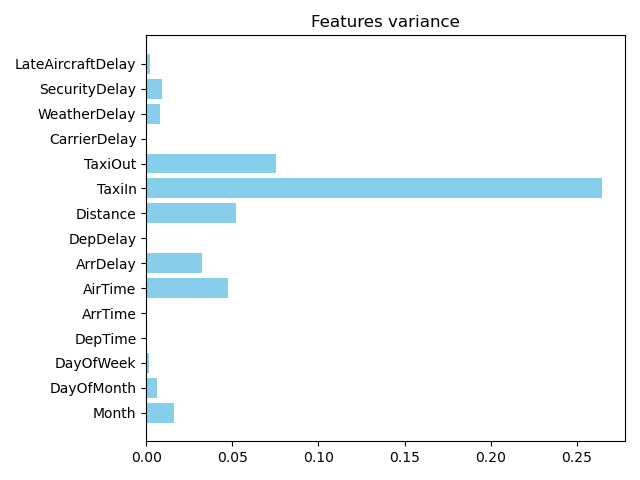
\includegraphics[scale=1]{images/balance_figure.png}
  \caption{}
  \label{fig:balance}
\end{figure}

Dans certains cas, cela semble cohérent avec des variations auxquelles on peut s'attendre Par exemple : Plus d'avions lors des vacances d'été et d'hiver [fig:\ref{fig:Month}] ou un équilibre entre les jours du mois. [fig:\ref{fig:DayOfMonth}]

\begin{figure}[H]
  \centering
  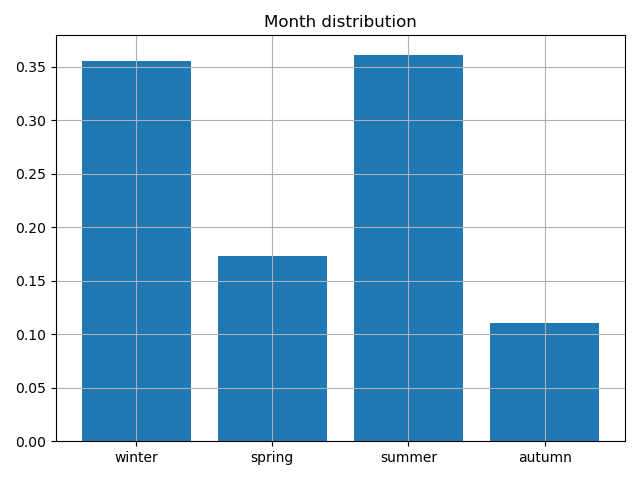
\includegraphics[scale=1]{images/Month_distribution.png}
  \caption{}
  \label{fig:Month}
\end{figure}

\begin{figure}[H]
  \centering
  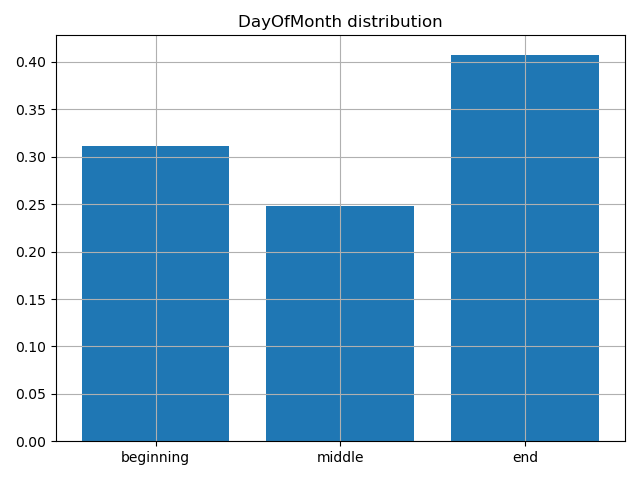
\includegraphics[scale=1]{images/DayOfMonth_distribution.png}
  \caption{}
  \label{fig:DayOfMonth}
\end{figure}

Dans d'autres cas, cela peut être plus étonnant. [fig:\ref{fig:TaxiIn}]
Ici, dans le cas des taxis cela peut indiquer, soit que les taxis déposent très rapidement les voyageurs, ce qui est possible, soit que les classes sont mal définies.
En effet, la modalité 'short' de 'TaxiIn' va jusqu'à 20 minutes d'attente, il serait donc potentiellement judicieux de rajouter une modalité intermédiaire à 'short' et 'medium' pour augmenter la granularité de la donnée, augmenter sa précision et son équilibre.

\begin{figure}[H]
  \centering
  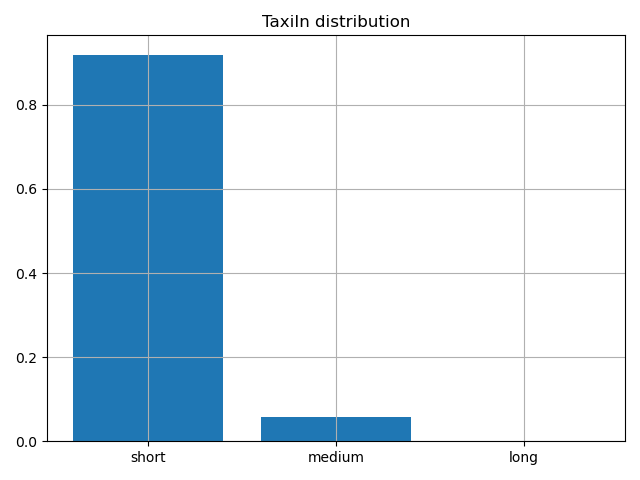
\includegraphics[scale=1]{images/TaxiIn_distribution.png}
  \caption{}
  \label{fig:TaxiIn}
\end{figure}

